% Intrinsic Efficiency
\documentclass[draftcls,onecolumn]{IEEEtran}

%% INCLUDING THE PREAMBLE
%%%%%%%%%%%%%%%%%%%%%%%%%%%%%%%%%%%%%%%%%%%%%%%%%%%%%%%%%%%%%%%%%%%%%%%%%%%
%                                                                         %
%                                 PREAMBLE                                %
%                                                                         %
%%%%%%%%%%%%%%%%%%%%%%%%%%%%%%%%%%%%%%%%%%%%%%%%%%%%%%%%%%%%%%%%%%%%%%%%%%%

%% PACKAGES
\usepackage[]{lineno}
%\linenumbers
\usepackage[usenames,dvipsnames]{xcolor}
\usepackage{microtype}
\usepackage[obeyDraft]{todonotes}
\usepackage{fancyvrb}
\VerbatimFootnotes
\usepackage{algorithmic}

%% GRAPHICS RELATED
\usepackage{graphicx}
\usepackage[outdir=./tmp/]{epstopdf}
\graphicspath{{../images/}{./}{./tmp/}}
\DeclareGraphicsExtensions{.eps, .pdf, .jpeg, .png,}

%% CPATION SETUP
\usepackage{float}
\usepackage{caption}
\usepackage{subcaption}
\captionsetup{belowskip=12pt,aboveskip=4pt}


%% BIBLIOGRAPHY
\bibliographystyle{ieeetr}

%% UNITS
\usepackage{siunitx}

%% EQUATIONS
\usepackage{amsmath}
%\numberwithin{equation}{section}

%% HYPERLINKS
\usepackage[debug]{hyperref}

%%%%%%%%%%%%%%%%%%%%%%%%%%%%%%%%%%%%%%%%%%%%%%%%%%%%%%%%%%%%%%%%%%%%%%%%%%%
%                                                                         %
%                             Listing Setup                               %
%                                                                         %
%%%%%%%%%%%%%%%%%%%%%%%%%%%%%%%%%%%%%%%%%%%%%%%%%%%%%%%%%%%%%%%%%%%%%%%%%%%
\usepackage{listings}
\lstset{ %
    language=C++,
    basicstyle=\footnotesize\ttfamily,
    numbers=left,
    numberstyle=\tiny\color{gray},
    stepnumber=2,
    numbersep=5pt,
    backgroundcolor=\color{white},
    showspaces=false,
    showstringspaces=false,
    showtabs=false,
    frame=single,
    rulecolor=\color{black},
    tabsize=2,
    breaklines=true,
    breakatwhitespace=false,
    title=\lstname,
    keywordstyle=\color{blue},
    commentstyle=\color{OliveGreen},
    stringstyle=\color{orange}
}
\DeclareCaptionFont{white}{\color{white}}
\DeclareCaptionFormat{listing}{\colorbox[cmyk]{0.43, 0.35, 0.35, 0.01}{\parbox{\dimexpr\textwidth-2\fboxsep\relax}{#1#2#3}}}
\captionsetup[lstlisting]{format=listing,labelfont=white,textfont=white,singlelinecheck=false,margin=0pt,font={bf,footnotesize}}
%\lstnewenvironment{code}[1][]%
%{ \noindent\minipage{\linewidth}
%	\lstset{#1}
%}
%{\endminipage}
%% USER COMMANDS
\usepackage{isotope}
\newcommand{\iso}{\isotope}
\newcommand{\figurewidth}{\textwidth}
\newcommand{\micron}{$\mu$m}


% index generation
\usepackage{makeidx}
\usepackage{exercise}
\makeindex
 
% 'list of notations' generation
\usepackage[refpage]{nomencl}  % refer to the page where notation appears
\newcommand{\definevar}[2]{#1 #2\nomenclature{#1}{#2}}
\renewcommand{\nomname}{List of Notations}
\renewcommand*{\pagedeclaration}[1]{\unskip\dotfill\hyperpage{#1}}
\makenomenclature
 


%% Start of the document
\begin{document}
\title{Intrinsic Efficiency Calculations}
\author{Matthew J. Urffer}
\date{\today}
\maketitle

% Nomenclature
\printnomenclature
\printindex

% Tables of Contents, Figures, Tables
\listoftodos
\tableofcontents
\listoffigures
\listoftables
\lstlistoflistings
\section{Intrinsic Efficiency}
Often times it is necessary to relate the performance of a detector to number of particles that cross the detector, this is completed using the intrinsic efficiency.
Thus the intrinsic efficiency it is a measure at how efficient the detector is at detecting radiation, normalized to the amount of radiation that crosses the detector.
The intrinsic efficiency is defined as the ratio between the counts recorded in the detector and the number of impingement radiation on the detector\cite{knoll_radiation_2009}, expressed as \eqref{eqn:intEffDef},
\begin{align}
  \label{eqn:intEffDef}
  \epsilon_{int} = \frac{N_c}{N_i}
\end{align}
where:
\begin{itemize}
  \item[] \definevar{$\epsilon_{int}$}{intrinsic efficiency},
  \item[] \definevar{$N_c$}{number of counts recorded by the detector}, and
  \item[] \definevar{$N_i$}{quanta of radiation incident upon the detector}.
\end{itemize}
In order to determine the intrinsic efficiency of a detector it is then necessary to determine the performance of the detector (easily completed by measuring the detector) and the number of radiation impingement upon the detector (usually accomplished through calculation on simulation).

The quanta of radiation incident upon the detector can be expressed as the product of two components: the source strength and the solid angle, \eqref{eqn:QuantaIncidentDef},
\begin{align}
  \label{eqn:QuantaIncidentDef}
  N_i = \Omega S_0
\end{align}
where:
\begin{itemize}
  \item[] \definevar{$S$}{source strength}, and 
  \item[] \definevar{$\Omega$}{fraction of solid angle detector subtends}.
\end{itemize}
Radiation sources generally decay from their initial source strength according to the half-life of the source.
The time dependent source strength, $S(t)$ can then be expressed as \eqref{eqn:HalfLife}, where \definevar{$S_0$}{initial source strength}, \definevar{$t_{1/2}$}{half life} and \definevar{$t$}{age of source}.
\begin{align}
  \label{eqn:HalfLife}
  S(t) = S_0 e^{-\frac{\ln{2}}{t_{1/2}} t}
\end{align}

The fraction of the source solid angle the detector subtends, $\Omega$, is computed using MCNPX. 
A F1 tally, defined in \eqref{eqn:F1Def}, is employed over the detector surface with two cosine bins, $-1<\cos\theta<0$ and $0<\cos\theta<1$, which divide the tally into particles that enter the surface and particles that leave the surface, respectively.
\begin{align}
  \label{eqn:F1Def}
  F1 &= \int_A dA \int_E dE \int_{4\pi} d\Omega ;;\vec{n}\cdot\vec{J}(\vec{r},E,\vec{\Omega}) \\
 %  &= \int_A dA \int_E dE \int_{4\pi} d\Omega \vec{n}\cdot\vec{\Omega}\Phi(\vec{r},E,\vec{\Omega}) \notag
\end{align}
In \eqref{eqn:F1Def} the position $\vec{r}$\nom{$\vec{r}$}{position}, direction $\vec{\Omega}$\nom{$\vec{\Omega}$}{direction} and energy $E$ \nom{$E$}{energy} dependent particle current $\vec{J}$ \nom{$\vec{J}$}{particle current} is integrated over the entire area, energy and direction normal to the surface of the area.
As macro-bodies are used for the surfaces of the detector, $-1<\cos\theta<0$ represents the particles that cross into the surface and $0<\cos\theta<1$ the particles that leave the surface.
In the case where macrobodies are not used to create the cell, the reader is referred to the MCNPX manual for more details.

The count rate of a detector is found by integrating the measured spectra, $p(x)$, \nom{$p(x)$}{measured spectra as a function of channel number $x$} over some bounds of integration.
It is then possible to express the intrinsic efficiency as a function of a mathematical lower level discriminator (MLLD) of the measured spectra \footnote{The MLLD behaves essentially as a physical lower level discriminator in that all counts below this value are discarded.} in order to determine at what MLLD the intrinsic efficiency is less then a value.
Equation \eqref{eqn:MLLDDef} shows such a formulation of the intrinsic efficiency as a function of a MLLD, where the upper bond is assumed to be the end of the spectra or highest recorded channel of the analog to digital converter.
\begin{align}
	\label{eqn:MLLDDef}
	\epsilon_{int}(MLLD) &= \frac{\int_{MLLD}^\infty p(x)dx}{N_i}
\end{align}

\subsection{Neutron Intrinsic Efficiency}
The number of counts upon a detector is measured by irradiating the detector in a lead and cadmium well of the neutron irridiator to determine $N_i$, and then simulating that geometry in bench-marked MCNPX in order to determine the number of neutrons incident on the detector\footnote{MCNPX simulations were benched-marked against GS20 and against polymer films, having 4\% and 15\% agreement to measured count rate, respectively.}.
The determination of $N_i$ consists of two parts: 1) determining the number of neutrons crossing the detector surface in the lead and cadmium wells and, 2) determining the source strength.
The \iso[252]{Cf} source was \SI{0.59}{\ug} on July 2, 2009.
Given that the half-life of \iso[252]{Cf} is 2.64 years and \iso[252]{Cf} has a spontaneous neutron emission rate of \SI{2.3E6}{neutron\per\second\per\micro\gram} the time dependent source strength can be calculated as \eqref{eqn:Cf252SourceStrength}.
\begin{align}
  \label{eqn:Cf252SourceStrength}
  S(t) &= S_0 e^{-\frac{\ln{2}}{t_{1/2}} t} \\ \notag 
    &= \SI{0.59}{\ug} \iso[252]{Cf} \;\frac{\SI{2.3E6}{neutron\per\second}}{\si{\ug} \iso[252]{Cf}}\; e^{-\frac{ \ln{2}}{\SI{2.64}{year}}t}  \\ \notag
    &= \SI{1.357E6}{neutron\per\second}\; e^{-\frac{ \ln{2}}{\SI{2.64}{year}}t} 
\end{align}

Table \ref{tab:NeutronSolidAngle} summarizes the incident flux for a number of different detector sizes and heights.
The fraction of solid angle subtended by other geometries can be computed by interpolation on the values of this table, as shown in the examples calculations.
It should be noted that there is considerable variation in the neutron flux in the detector wells, as shown in Figure \ref{fig:NeutronFluxProfiles}.
Thus, even though the calculations are accurate to less than a percent, the physical error on the intrinsic efficiency will be much higher due to uncertainty in where the detector was placed in the well.

\begin{table}
	\centering
	\caption[Simulated Thermal Neutron Solid Angle for Various Film Radii]{Simulated Neutron Solid Angle for Various Film Radii in the net spectra. The film radii are shown in seperate columns, with the thickness in rows. The thermal spectra (shown) is the subtraction of the lead and cadmium wells.}
	\label{tab:NeutronSolidAngle}
	\begin{tabular}{c | c c c c c c}
Thickness (\si{\cm})	&	\SI{1}{\cm}	&	\SI{1.27}{\cm}	&	\SI{1.905}{\cm}	&	\SI{2}{\cm}	&	\SI{2.5}{\cm}	&	\SI{2.54}{\cm} \\ \hline
0.0025	&	0.00055	&	0.00089	&	0.00204	&	0.00225	&	0.00351	&	0.00362	\\
0.005	&	0.00055	&	0.00090	&	0.00204	&	0.00224	&	0.00350	&	0.00361	\\
0.01	&	0.00055	&	0.00089	&	0.00204	&	0.00223	&	0.00348	&	0.00359	\\
0.015	&	0.00055	&	0.00089	&	0.00202	&	0.00222	&	0.00346	&	0.00357	\\
0.03	&	0.00056	&	0.00090	&	0.00201	&	0.00221	&	0.00341	&	0.00353	\\
0.1	&	0.00058	&	0.00093	&	0.00202	&	0.00220	&	0.00334	&	0.00347	\\
0.2	&	0.00063	&	0.00099	&	0.00208	&	0.00225	&	0.00338	&	0.00349	\\
0.5	&	0.00080	&	0.00119	&	0.00234	&	0.00251	&	0.00365	&	0.00375	\\
1	&	0.00109	&	0.00159	&	0.00286	&	0.00306	&	0.00427	&	0.00437	\\
2	&	0.00170	&	0.00233	&	0.00389	&	0.00412	&	0.00544	&	0.00555	\\
	\end{tabular}
\end{table}
\begin{figure}
	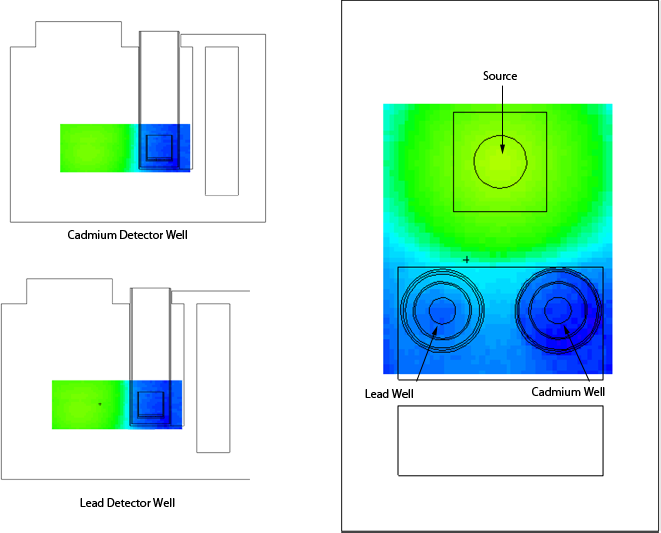
\includegraphics[width=\textwidth]{SpatialNeutronFlux}
  \caption[Neutron Flux Profiles of the Lead and Cadmium Wells]{Neutron Flux Profiles of the Lead and Cadmium Wells. Lighter colors correspond to a higher neutron population. The effect of the cadmium shielding is observed in the depression of the flux in the lower right by the cadmium well.}
  \label{fig:NeutronFluxProfiles}
\end{figure}

\subsection{Gamma Intrinsic Efficiency}
The gamma irridiator consists of a \SI{97}{\micro Ci} \iso[60]{Co} (January 1st, 2012) inside of a steel pipe encased in lead bricks.
The gamma intrinsic efficiency is calculated by simulating the fraction of solid angle the detector subtends and then using radioactive decay to model the \iso[60]{Co} source.
The \iso[60]{Co} source strength is calculated according to \eqref{eqn:Co60SourceStrength}. 
As there are two photons emitted from each \iso[60]{60} decay, in order to normalize the MCNPX source strength it is necessary to multiply the single photon activity by two.
Tabulated solid angle fractions are in Table \ref{tab:GammaSolidAngle}, and once again interpolation can be used for geometries not enumerated.
These values were extracted from an MCNPX simulation using an F1 tally as described above.
\begin{align}
  \label{eqn:Co60SourceStrength}
  S &= S_0 e^{-\frac{\ln{2}}{t_{1/2}} t} \\ \notag 
    &= \SI{97}{\micro Ci} \iso[60]{Co}\; \frac{\SI{3.7E10}{decay\per\second}}{\si{Ci}} \;\frac{2\text{photon}}{decay}\;e^{-\frac{ \ln{2}}{\SI{5.27}{year}}t}  \\ \notag
    &= \SI{7.178E6}{photon\per\second}\;e^{-\frac{ \ln{2}}{\SI{5.27}{year}}t} 
\end{align}
\begin{table}
	\centering
	\caption{Simulated Gamma Solid Angle for Various Film Radii}
	\label{tab:GammaSolidAngle}
	\begin{tabular}{c | c c c c c c}
Thickness (\si{\cm})	&	\SI{1}{\cm}	&	\SI{1.27}{\cm}	&	\SI{1.905}{\cm}	&	\SI{2}{\cm}	&	\SI{2.5}{\cm}	&	\SI{2.54}{\cm} \\ \hline
0.0025	&	0.0060	&	0.0095	&	0.0206	&	0.0226	&	0.0347	&	0.0357\\
0.005	&	0.0060	&	0.0095	&	0.0206	&	0.0226	&	0.0347	&	0.0357\\
0.01	&	0.0060	&	0.0095	&	0.0206	&	0.0226	&	0.0347	&	0.0357\\
0.015	&	0.0060	&	0.0095	&	0.0206	&	0.0226	&	0.0347	&	0.0357\\
0.03	&	0.0060	&	0.0095	&	0.0206	&	0.0227	&	0.0347	&	0.0357\\
0.1	&	0.0060	&	0.0096	&	0.0207	&	0.0227	&	0.0348	&	0.0358\\
0.2	&	0.0061	&	0.0097	&	0.0209	&	0.0229	&	0.0349	&	0.0360\\
0.5	&	0.0063	&	0.0099	&	0.0212	&	0.0232	&	0.0353	&	0.0364\\
1	&	0.0066	&	0.0103	&	0.0217	&	0.0237	&	0.0359	&	0.0379\\
2	&	0.0071	&	0.0109	&	0.0225	&	0.0247	&	0.0371	&	0.0382\\
3	&	0.0075	&	0.0114	&	0.0233	&	0.0255	&	0.0381	&	0.0392\\
4	&	0.0079	&	0.0119	&	0.0240	&	0.0262	&	0.0390	&	0.0401\\
	\end{tabular}
\end{table}
It should be noted that the gamma irridiator detector well is encased in a 1/2 inch steel pipe which is surrounded by lead, providing a beam like geometry while also introducing lower energy photons. 
The contribution of these lower energy photons is shown in Figure \ref{fig:PhotonFluxAllEnergies}, and it is evident that these contributions are a magnitude less than the contributions from the primary photons of the \iso[60]{Co} decay.
\begin{figure}
  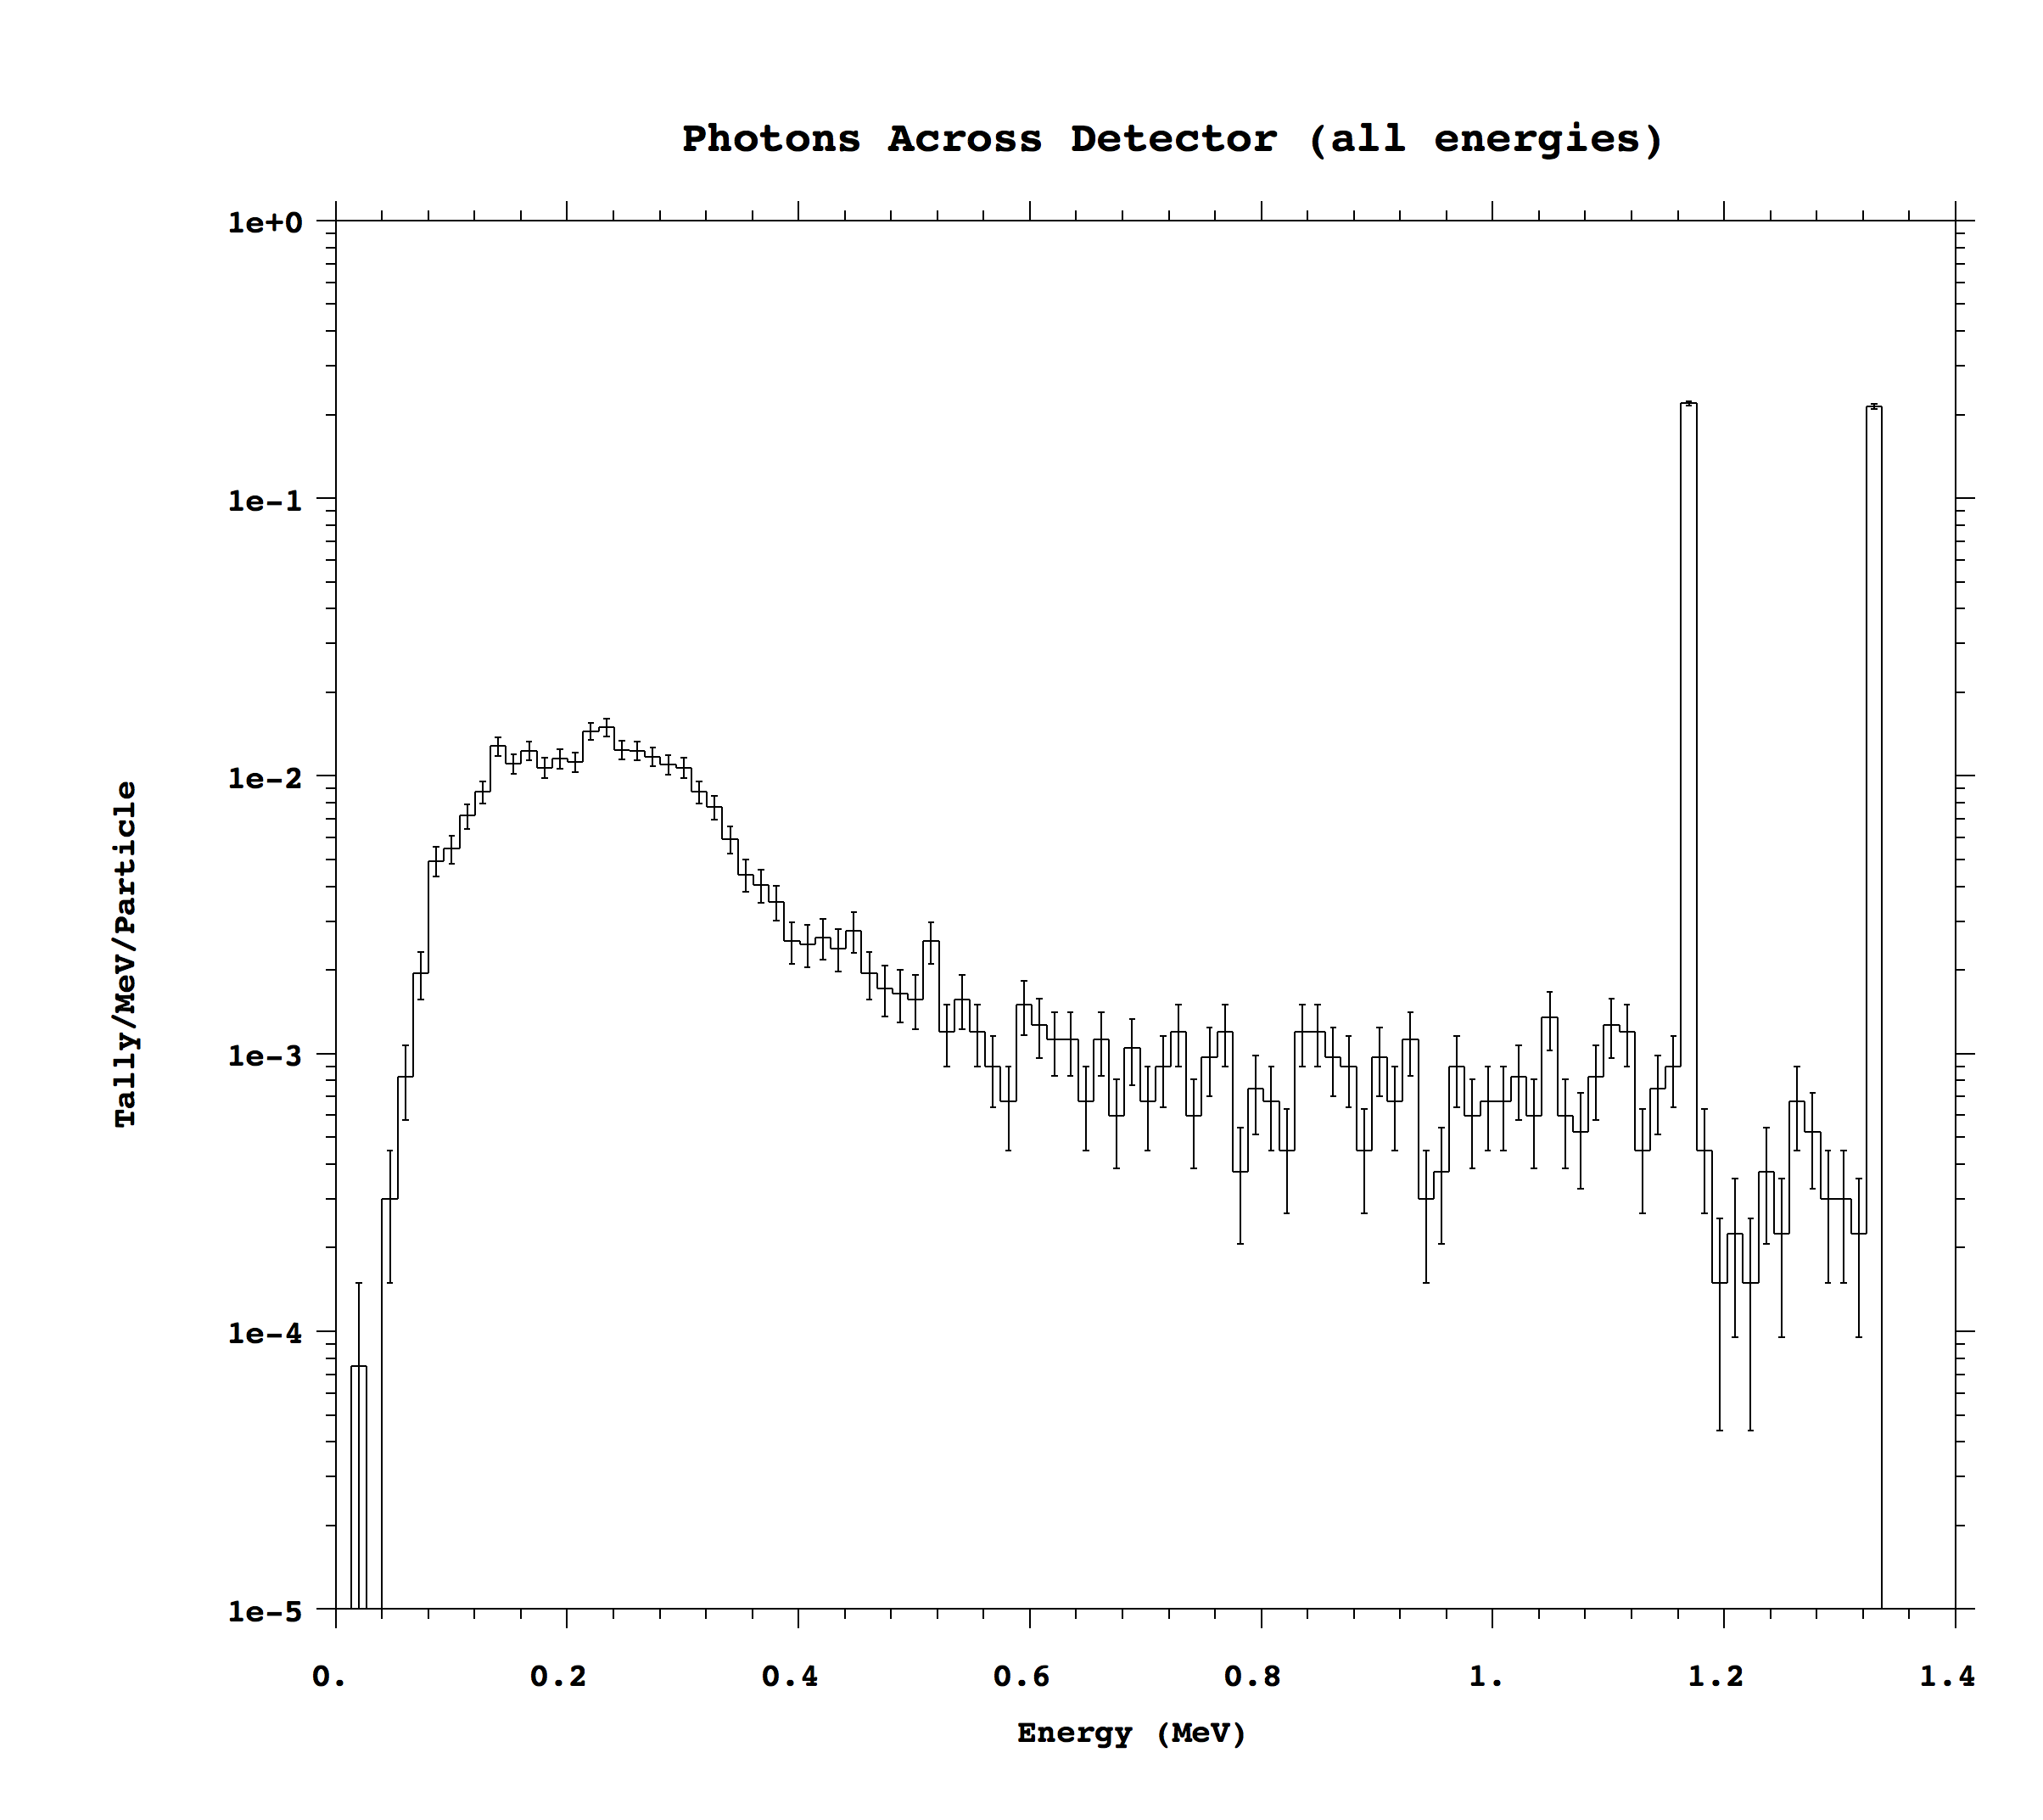
\includegraphics[width=\textwidth]{PhotonEnergyDist}
	\caption[Photons Incident upon Detector]{Photons incident upon a detector from an \iso[60]{Co} source.  The two \iso[60]{Co} photons (\SI{1.17}{\MeV} and \SI{1.33}{\MeV}) make up the majority of the incident photons.}
  \label{fig:PhotonFluxAllEnergies}
\end{figure}
Table \ref{tab:GammaSolidAngle} considers the contributions from all sides, but it is evident that the contributions from the side scattering is not large as 100 times increase in the thickness (\SI{50}{\um} to \SI{5}{\mm}) results in only a 4\% increase in the number of particles crossing the detector.

\pagebreak
\subsection{Examples}
\begin{Exercise*}[label={LiBorateGlass},title={Li borate glass},name={Example}]
A \SI{1.327}{\g} sample of $\iso[6]{Li}\text{B}_4\text{O}_7$ glass was fabricated by John Auxier was measured on April 4, 2013.
This sample was roughly rectangular in shape (\SI{1.3}{\cm} by \SI{2.2}{\cm}) with a thickness of \SI{2.7}{\mm}.
The neutron intrinsic efficiency is calculated according to \eqref{eqn:intEffDef} with the source strength as supplied in \eqref{eqn:Cf252SourceStrength}, and the source aging $t = 3.76 \text{yr}$.
\begin{align}
    S &= \SI{1.357E6}{neutron\per\second} e^{-\frac{ \ln{2}}{\SI{2.64}{year}}\SI{3.76}{year}} \\ \notag
      &= \SI{5.06E5}{neutron\per\second}
\end{align}
Approximating the sample as a cylinder (maintaining the area of the faces) yields a radius of \SI{0.95}{\cm}.
\begin{align}
	r &= \sqrt{\frac{\SI{1.3}{\cm} \times \SI{2.2}{\cm}}{\pi}} \\ \notag
	& = \SI{0.95}{\cm}
\end{align}
From Table \ref{tab:NeutronSolidAngle} the closest radius is \SI{1}{\cm}.
Linear interpolation is used to calculate the expected solid angle at a thickness of \SI{0.27}{\cm}, and then a ratio of the areas is used to calculate the solid angle at a radius of \SI{0.95}{\cm}.
\begin{align*}
	\frac{A_1}{A_2} &= \frac{\Omega_1}{\Omega_2} \\ 
	\Omega_2 &= \frac{r_2^2 \Omega_2}{r_1^2} \\
	 &= \frac{\SI{0.95}{\cm}^2 \num{6.73E-4}}{\SI{1}{\cm}^2}\\
	 &= \num{6.07E-4}
\end{align*}
This is then multiplied by the source strength on the date of the measurement, \SI{5.06E5}{neutron\per\second}, to determine the number of neutrons incident upon the detector in the thermal neutron measurement.
\begin{align*}
 	N_i &= \Omega S \\
	 &= \left (\num{6.07E-4}\right) \;\left( \SI{5.06E5}{neutron\per\second}\right) \\
   &= \SI{306}{neutron\per\second}
\end{align*}

The \iso[60]{Co} source has aged 459 days (1.26 years) from it purchased activity to the date of measurement.
The source strength is then:
\begin{align}
  S &= \SI{7.178E6}{photon\per\second}\;e^{-\frac{ \ln{2}}{\SI{5.27}{year}}\SI{1.26}{year}} \\ \notag
    &= \SI{6.08E6}{photon\per\second}
\end{align}
Once again interpolation is used to calculated the solid angle.
\begin{align*}
	\frac{A_1}{A_2} &= \frac{\Omega_1}{\Omega_2} \\ \notag
	\Omega_2 &= \frac{r_2^2 \Omega_2}{r_1^2} \\
	 &= \frac{\SI{0.95}{\cm}^2 \num{6.17E-3}}{\SI{1}{\cm}^2} \\
	 &= \num{5.57E-3}
\end{align*}
This is then multiplied by the source strength on the date of the measurement, \SI{6.08E6}{photon\per\second}, to determine the flux.
\begin{align*}
 	N_i &= \Omega S \\
	 &= \num{5.57E-3} \; \SI{6.08E6}{photon\per\second} \\
      &= \SI{3.39E4}{neutron\per\second}
\end{align*}
It is then possible to plot the intrinsic efficiency in your favorite computational package.

\end{Exercise*}
\begin{Exercise*}[label={LiquidSample},title={Liquid Sample},name={Example}]
The neutron fluence over a \SI{5}{\milli\liter} vial is desired in order to compute the intrinsic efficiency of neutron samples fabricated and measured by members of SCSU.
MCNPX calculations for the solid angle, $\Omega$ show that \SI{4.477E-3}{neuron\per source particle} cross the sample in the lead well, and \SI{1.475E-3}{neutron\per source particle} cross the sample in the cadmium well.
Thus the net particles crossing the detector is $\Omega_{\text{net}} =\SI{4.477E-3}{neuron\per source particle} - \SI{1.475E-3}{neuton\per source particle} =\SI{3.002E-3}{neuton\per source particle} $.
Depending on when the sample was measured the number of neutrons crossing the sample can be calculated by multiply \eqref{eqn:Cf252SourceStrength} by the solid angle calculated above.

Thus, for a sample measured August 8, 2012 the net neutron fluence over the vial is  \SI{1.80E3}{neutron\per\second}.
This was compared to the fluence calculated by assuming a neutron flux of \SI{530}{neutron\per\second\per\cm\squared} on July 2, 2009, with the area of the vial being \SI{45}{\cm\squared}.
This yield a fluence of \SI{5.98E3}{neutron\per\second}, which is 3.3 times higher than the fluence as calculated by an F1 tally.
However, depending on how the flux was calculated it probably including contributions from particles leaving and entering the detector volume, while the calculation based on the solid angle only considers particles entering the detector.
In addition, the flux is not isotropic over the entire detector, which the above calculation in which it is multiplied by the surface area assumes.
Thus, it is is determined that the two methods are roughly equivalent.


The SCSU samples where not measured in the \iso[60]{Co} irridiator but rather by placing a source on the outside of the sample.

\end{Exercise*}

% Bibliography
\bibliography{../Zotero}

\pagebreak
\appendices
\section{Code Listings}
The generated MCNPX tables was based upon a script input deck for gamma and neutrons in \path{/home/murffer/MCNP/IncidentFlux}.
The bash shell script necessary to run the different simulations is shown in Listing \ref{lst:RUNDATA}. 
The accompanying Torque/MAUI submission scripts are shown in Listings \ref{lst:nSub} and \ref{lst:gSub}.
%%%%%%%%%%%%%%%%%%%%%%%%% LISTING CODE %%%%%%%%%%%%%%%%%%%%%%%%%%
\lstinputlisting[language=bash,caption=Main Run Script,label=lst:RUNDATA]{RUNDATA.sh}
\lstinputlisting[language=bash,caption=Neutron Submission Script,label=lst:nSub]{nRunScript.sh}
\lstinputlisting[language=bash,caption=Gamma Submission Script,label=lst:gSub]{gRunScript.sh}
An analysis script was written in python in order to extract the necessary lines from the output decks, and is shown in Listing \ref{lst:Analysis}.
The output of the this script is two excel files (one for the gamma irridiator and the other for the neutron irridiator) which contain the fraction of the solid angle that the detector subtends.
%%%%%%%%%%%%%%%%%%%%%%%%% LISTING CODE %%%%%%%%%%%%%%%%%%%%%%%%%%
\lstinputlisting[caption=Python Analysis Script,label=lst:Analysis]{analysis.py}

Listing \ref{lst:MillerConfig} is the MCNPX input deck for the neutron irridiator, while Listing \ref{lst:GammaConfig} is the input deck for the gamma irridiator.
%%%%%%%%%%%%%%%%%%%%%%%%% LISTING CODE %%%%%%%%%%%%%%%%%%%%%%%%%%
\lstinputlisting[caption=MCNP Input Deck of Neutron Irridiator,label=lst:MillerConfig]{Miller-Config_Script.mcnp}
%%%%%%%%%%%%%%%%%%%%%%%%% LISTING CODE %%%%%%%%%%%%%%%%%%%%%%%%%%
\lstinputlisting[caption=MCNP Input Deck of Gamma Irridiator,label=lst:GammaConfig]{Script_Irridiator.mcnp}
\end{document}

